\documentclass[crop,tikz]{standalone}

\usepackage{makecell}

\definecolor{alizarin}{rgb}{0.82, 0.1, 0.26}
\definecolor{airforceblue}{rgb}{0.36, 0.54, 0.66}
\definecolor{apricot}{rgb}{0.98, 0.81, 0.69}
\definecolor{blush}{rgb}{0.87, 0.36, 0.51}
\definecolor{cadmiumgreen}{rgb}{0.0, 0.42, 0.24}
\definecolor{cambridgeblue}{rgb}{0.64, 0.76, 0.68}
\definecolor{celadon}{rgb}{0.67, 0.88, 0.69}
\definecolor{chestnut}{rgb}{0.8, 0.36, 0.36}
\definecolor{harvardcrimson}{rgb}{0.79, 0.0, 0.09}
\definecolor{darkseagreen}{rgb}{0.56, 0.74, 0.56}
\definecolor{aoenglish}{rgb}{0.0, 0.5, 0.0}
\definecolor{brightube}{rgb}{0.82, 0.62, 0.91}

\usetikzlibrary{positioning}
\usetikzlibrary{matrix}
\usetikzlibrary{fit}
\usetikzlibrary{calc,decorations.pathmorphing,patterns}

\newcommand{\vvector}[1]{\tikz{\draw[#1,step=1em,fill=#1!50] (0,0)  grid (1em,4em) rectangle (0, 0);}}
\newcommand{\hvector}[1]{\tikz{\draw[#1,step=1em,fill=#1!50] (0,0)  grid (4em,1em) rectangle (0, 0);}}
\newcommand{\vvectorSmall}[1]{\tikz{\draw[#1,step=.5em,fill=#1!50] (0,0)  grid (.5em,1.5em) rectangle (0, 0);}}

\newdimen\XCoord
\newdimen\YCoord
\newdimen\XXCoord
\newdimen\YYCoord

\newcommand{\outgoing}[2]{
  \path (#1); \pgfgetlastxy{\XCoord}{\YCoord};
  \path (#2); \pgfgetlastxy{\XXCoord}{\YYCoord};
  \draw[->, line width=1pt] (\XCoord, \YCoord) -- (\XCoord, \YYCoord);
}%
\newcommand{\incoming}[2]{
  \path (#1); \pgfgetlastxy{\XCoord}{\YCoord};
  \path (#2); \pgfgetlastxy{\XXCoord}{\YYCoord};
  \draw[->, line width=1pt] (\XCoord, \YYCoord) -- (\XCoord, \YCoord);
}%

\usetikzlibrary{calc}

\tikzset{
    ncbar angle/.initial=-90,
    ncbar/.style={
        to path=(\tikztostart)
        -- ($(\tikztostart)!#1!\pgfkeysvalueof{/tikz/ncbar angle}:(\tikztotarget)$)
        -- ($(\tikztotarget)!($(\tikztostart)!#1!\pgfkeysvalueof{/tikz/ncbar angle}:(\tikztotarget)$)!\pgfkeysvalueof{/tikz/ncbar angle}:(\tikztostart)$)
        -- (\tikztotarget)
    },
    ncbar/.default=0.5cm,
}

\begin{document}

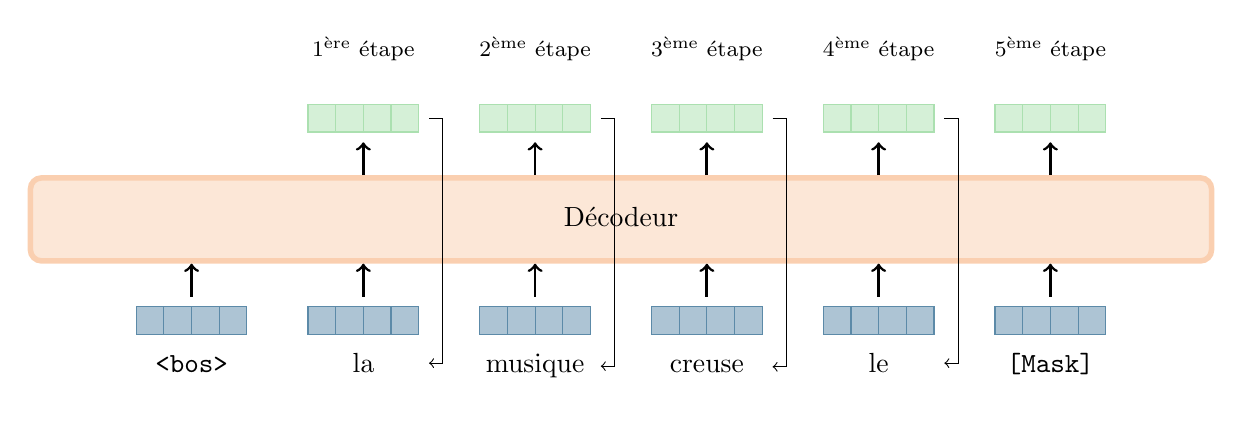
\begin{tikzpicture}[ampersand replacement=\&]
    \tikzset{node distance = .3cm and 2cm}

    \matrix (input) [matrix of nodes,
                     column sep=1.5em,
                     minimum width=2em,]
            { \hvector{airforceblue} \&
              \hvector{airforceblue} \&
              \hvector{airforceblue} \&
              \hvector{airforceblue} \&
              \hvector{airforceblue} \&
              \hvector{airforceblue} \\
              \texttt{<bos>} \& la \& musique \& creuse \& le \& \texttt{[Mask]} \\
            };

    \node [above=of input, minimum height=3em, minimum width=15cm, draw=apricot, rounded corners, line width=2pt, fill=apricot!50] (transformer) {\makecell{Décodeur}};

    \matrix (output) [matrix of nodes,
                      column sep=1.5em,
                      above=of transformer,
                      minimum width=2em,]
            {
              \hvector{white}   \&
              \hvector{celadon} \&
              \hvector{celadon} \&
              \hvector{celadon} \&
              \hvector{celadon} \&
              \hvector{celadon} \\
            };

%    \incoming{output-1-1.south}{transformer.north}
    \incoming{output-1-2.south}{transformer.north}
    \incoming{output-1-3.south}{transformer.north}
    \incoming{output-1-4.south}{transformer.north}
    \incoming{output-1-5.south}{transformer.north}
    \incoming{output-1-6.south}{transformer.north}

    \outgoing{input-1-1.north}{transformer.south}
    \outgoing{input-1-2.north}{transformer.south}
    \outgoing{input-1-3.north}{transformer.south}
    \outgoing{input-1-4.north}{transformer.south}
    \outgoing{input-1-5.north}{transformer.south}
    \outgoing{input-1-6.north}{transformer.south}

%    \node [right=of input-1-5] {\makecell{\initial}};
%    \node [right=of output-1-5] {\makecell{\final}};

    \pgfpointanchor{input-2-2}{east}
    \pgfgetlastxy{\dummy}{\myy}
    \pgfpointanchor{input-1-2}{east}
    \pgfgetlastxy{\myx}{\dummy}
    \draw[->] (output-1-2.east) to [ncbar=-.5em] (\myx, \myy);

    \pgfpointanchor{input-2-3}{east}
    \pgfgetlastxy{\dummy}{\myy}
    \pgfpointanchor{input-1-3}{east}
    \pgfgetlastxy{\myx}{\dummy}
    \draw[->] (output-1-3.east) to [ncbar=-.5em] (\myx, \myy);

    \pgfpointanchor{input-2-4}{east}
    \pgfgetlastxy{\dummy}{\myy}
    \pgfpointanchor{input-1-4}{east}
    \pgfgetlastxy{\myx}{\dummy}
    \draw[->] (output-1-4.east) to [ncbar=-.5em] (\myx, \myy);

    \pgfpointanchor{input-2-5}{east}
    \pgfgetlastxy{\dummy}{\myy}
    \pgfpointanchor{input-1-5}{east}
    \pgfgetlastxy{\myx}{\dummy}
    \draw[->] (output-1-5.east) to [ncbar=-.5em] (\myx, \myy);

    \node [above=of output-1-2.north] {\footnotesize 1\textsuperscript{ère} étape};
    \node [above=of output-1-3.north] {\footnotesize 2\textsuperscript{ème} étape};
    \node [above=of output-1-4.north] {\footnotesize 3\textsuperscript{ème} étape};
    \node [above=of output-1-5.north] {\footnotesize 4\textsuperscript{ème} étape};
    \node [above=of output-1-6.north] {\footnotesize 5\textsuperscript{ème} étape};

\end{tikzpicture}

\end{document}